\documentclass[11pt]{article}

\usepackage[margin=1in]{geometry}
\usepackage[T1]{fontenc}
\usepackage{newpxtext,newpxmath}
\usepackage{microtype}
\usepackage{amsmath}
\usepackage{booktabs}
\usepackage{tabularx}
\usepackage{enumitem}
\usepackage{xcolor}
\usepackage{caption}
\usepackage{fancyhdr}
\usepackage{listings}
\usepackage{tikz}
\usetikzlibrary{arrows.meta,positioning,fit,calc,decorations.pathreplacing}
\usepackage[breakable,skins]{tcolorbox}
\usepackage[colorlinks=true,linkcolor=blue!50!black,citecolor=green!40!black,urlcolor=blue!60!black]{hyperref}

\setlist{itemsep=2pt,topsep=4pt}
\setlength{\parskip}{4pt}
\setlength{\emergencystretch}{2em}

\definecolor{vis}{HTML}{3B7DD8}
\definecolor{proj}{HTML}{8E5CD9}
\definecolor{llm}{HTML}{D9822B}
\definecolor{act}{HTML}{2E9E5B}
\definecolor{frz}{HTML}{888780}

\newtcolorbox{mental}[1][]{breakable,enhanced,colback=act!6,colframe=act!70!black,
  fonttitle=\bfseries,title={Mental model#1}}
\newtcolorbox{interp}[1][]{breakable,enhanced,colback=llm!6,colframe=llm!80!black,
  fonttitle=\bfseries,title={Interpretability note#1}}
\newtcolorbox{pitfall}[1][]{breakable,enhanced,colback=red!4,colframe=red!60!black,
  fonttitle=\bfseries,title={Common misconception#1}}

\lstset{basicstyle=\ttfamily\small,columns=fullflexible,frame=single,
  framerule=0.3pt,rulecolor=\color{black!30},backgroundcolor=\color{black!3},
  keywordstyle=\color{blue!60!black},commentstyle=\color{black!50},
  breaklines=true,showstringspaces=false,language=Python}

\pagestyle{fancy}
\fancyhf{}
\lhead{\small Fine-Tuning OpenVLA, and Fine-Tuning the Lens}
\rhead{\small\thepage}

\newcommand{\dm}{d_{\text{model}}}
\newcommand{\KL}{D_{\mathrm{KL}}}

\title{\textbf{Fine-Tuning OpenVLA, and Fine-Tuning the Lens}\\[4pt]
\large A study guide to adapting OpenVLA (full fine-tuning, LoRA, the LIBERO recipe)\\
and to \emph{trained read-outs} (tuned lens, probes) for the perception$\to$action question}
\author{Prepared for the VLAinterp project}
\date{October 2026}

\begin{document}
\maketitle
\thispagestyle{empty}

\begin{abstract}
\noindent ``Fine-tuning'' means two different things in this project, and mixing them up is the fastest way to get confused. \emph{Fine-tuning the model} changes OpenVLA's weights so it behaves differently: this is how the base model became the LIBERO-Spatial checkpoint you study. \emph{Fine-tuning a lens} trains a small read-out on top of a \emph{frozen} OpenVLA, so you can measure what is already inside it. The model itself never changes. This guide covers both, in four parts: (I)~what fine-tuning is mechanically, with a gradient-descent refresher; (II)~how OpenVLA itself is fine-tuned: the strategies the authors compared, LoRA in detail, the released LIBERO configuration, and what that implies for interpretability; (III)~lenses as trained read-outs: why the logit lens can mislead, how the tuned lens \cite{belrose2023tuned} fixes it, and how it relates to linear probes; (IV)~a concrete plan for using a tuned lens to test the perception$\to$action split suggested by your run~2 logit-lens results, including controls, the data you already have, and code sketches.
\end{abstract}

\tableofcontents
\newpage

%=====================================================================
\part{What Fine-Tuning Is}
%=====================================================================

\section{The one-paragraph mental model}

\begin{mental}[: fine-tuning]
\textbf{Fine-tuning is just more training, starting from weights that already work.} You keep the same machinery as the original training: a loss, gradients, an optimizer. You change three things: \emph{where you start} (pretrained weights, not random ones), \emph{what data you use} (a smaller, task-specific set), and \emph{which weights are allowed to move} (all of them, some of them, or new small add-on weights).
\end{mental}

The last choice is what separates the two meanings of fine-tuning in this project:

\begin{center}
\begin{tabularx}{\linewidth}{@{}lXX@{}}
\toprule
 & Fine-tuning the model & Fine-tuning a lens \\
\midrule
Goal & Change what the robot \emph{does} & Measure what the model \emph{already computes} \\
What moves & OpenVLA's own weights (or LoRA add-ons merged into them) & Only new read-out weights, e.g.\ one translator per layer \\
OpenVLA afterwards & A different model (new checkpoint) & Exactly the same model, bit for bit \\
Loss & Cross-entropy on demonstration actions & Usually KL to the model's \emph{own} final prediction \\
Example & Base OpenVLA $\to$ \texttt{openvla-7b-finetuned-\allowbreak libero-spatial} & Logit lens $\to$ tuned lens \\
\bottomrule
\end{tabularx}
\end{center}

\begin{pitfall}[: ``fine-tune the logit lens'' means ``fine-tune $W_U$'']
Not quite. $W_U$ is part of OpenVLA. Retraining it would change the model you are trying to study. When people say ``fine-tune the logit lens'', they almost always mean training \emph{extra} parameters that sit in front of a frozen $W_U$, one set per layer. This is the tuned lens (Part~III). The original $W_U$ is reused unchanged.
\end{pitfall}

\section{Gradient descent refresher}

Every kind of training in this document, model or lens, runs the same loop:

\begin{enumerate}
  \item \textbf{Forward pass.} Run a batch of examples through the network and compute the predictions.
  \item \textbf{Loss.} One number measuring how wrong the predictions are: cross-entropy for OpenVLA, KL divergence for a tuned lens.
  \item \textbf{Backward pass.} Compute the gradient $\nabla_\theta \mathcal{L}$: for every trainable number $\theta_i$, which direction to move it to reduce the loss.
  \item \textbf{Update.} Move each trainable number a small step against its gradient. The \emph{optimizer} (SGD, Adam, AdamW) decides the exact step, and the \emph{learning rate} sets its size.
\end{enumerate}

\begin{center}
\begin{tabularx}{\linewidth}{@{}lX@{}}
\toprule
Term & Meaning \\
\midrule
Trainable / frozen & In PyTorch, \texttt{requires\_grad=True} or \texttt{False}. Frozen weights still take part in the forward pass, but no gradient updates them. \\
Batch, step & A batch is the set of examples in one forward/backward pass. A step is one update. \\
Epoch & One full pass over the training data. \\
Learning rate (LR) & Step size. Too large and training diverges; too small and nothing changes. \\
AdamW & Adam (per-parameter adaptive step sizes with momentum) plus decoupled weight decay. The default for transformers. \\
Weight decay & A pull toward zero (or toward an initial value) on every update. It discourages large, overfit weights. \\
Held-out set & Examples never used for updates. They are the only honest measure of whether training generalizes. \\
\bottomrule
\end{tabularx}
\end{center}

\begin{mental}[: frozen vs.\ trainable]
A frozen network is like a camera bolted to a tripod. You can still take pictures with it (forward passes), and you can learn to \emph{interpret} its pictures better (train a lens), but nothing you do changes the camera. Fine-tuning the model means unbolting the camera and adjusting it.
\end{mental}

%=====================================================================
\part{Fine-Tuning OpenVLA Itself}
%=====================================================================

\section{The menu of strategies}

OpenVLA's authors compared ways to adapt the pretrained model to a new robot setup (Franka tasks, batch size 16) \cite{kim2024openvla}:

\begin{center}
\begin{tabular}{@{}lrrr@{}}
\toprule
Strategy (what is trainable) & Success & Trainable params & VRAM \\
\midrule
Full fine-tuning (everything) & $69.7\pm7.2\%$ & 7{,}188.1M & 163.3 GB \\
Last layer only & $30.3\pm6.1\%$ & 465.1M & 51.4 GB \\
Frozen vision (everything but the encoders) & $47.0\pm6.9\%$ & 6{,}760.4M & 156.2 GB \\
Sandwich (vision + token embeddings + last layer) & $62.1\pm7.9\%$ & 914.2M & 64.0 GB \\
\textbf{LoRA, $r=32$} & $\mathbf{68.2\pm7.5\%}$ & \textbf{97.6M (1.4\%)} & 59.7 GB \\
LoRA, $r=64$ & $68.2\pm7.8\%$ & 195.2M & 60.5 GB \\
\bottomrule
\end{tabular}
\end{center}

\paragraph{How to read this.}
\begin{itemize}
  \item \textbf{Training only the last layer fails} (30\%). Adapting to a new robot needs changes throughout the network, not just at the read-out.
  \item \textbf{Freezing the vision encoders hurts badly} (47\%). The same lesson as in pretraining: robot control needs visual features the encoders don't produce out of the box.
  \item \textbf{LoRA matches full fine-tuning} while training 1.4\% of the parameters, on one GPU in 10--15 hours. Going from rank 32 to 64 buys nothing. Every released LIBERO checkpoint uses LoRA $r=32$.
\end{itemize}

\section{LoRA, in detail}

\subsection{The idea}
LoRA (Low-Rank Adaptation) \cite{hu2021lora} freezes every original weight matrix $W$ and learns a \emph{low-rank correction} next to it:
\begin{equation}
W_{\text{eff}} = W + \frac{\alpha}{r}\, B A,
\qquad A\in\mathbb{R}^{r\times d_{\text{in}}},\;\; B\in\mathbb{R}^{d_{\text{out}}\times r},\;\; r \ll d.
\end{equation}
\begin{itemize}
  \item $A$ squeezes the input down to $r$ numbers, and $B$ expands them back. Their product $BA$ has the same shape as $W$ but rank at most $r$.
  \item \textbf{$B$ starts at zero}, so $BA=0$ and the model starts out exactly equal to the pretrained one. $A$ starts random. (PEFT's default is Kaiming-uniform; OpenVLA sets \texttt{init\_lora\_weights="gaussian"}.)
  \item $\alpha/r$ is a fixed scale that keeps update sizes comparable across ranks.
  \item \textbf{Why it works:} the change needed to adapt a pretrained model tends to be low-dimensional. You don't need 16.8M free numbers to nudge a $4096\times4096$ matrix toward a new task.
\end{itemize}

\begin{figure}[h]
\centering
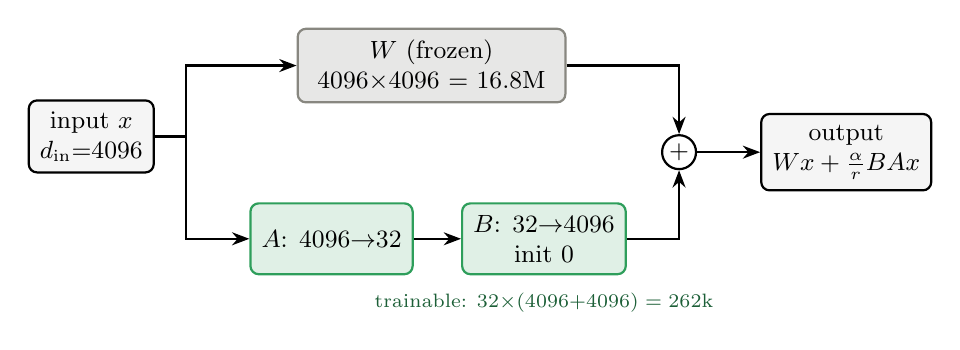
\begin{tikzpicture}[font=\small,
  box/.style={draw,rounded corners=3pt,thick,minimum height=9mm,align=center,inner sep=4pt},
  arr/.style={-{Stealth[length=2.2mm]},thick}]
\node[box,fill=black!4] (x) {input $x$\\$d_{\text{in}}{=}4096$};
\node[box,fill=frz!20,draw=frz,right=18mm of x,yshift=9mm,minimum width=34mm] (W) {$W$ (frozen)\\$4096{\times}4096$ = 16.8M};
\node[box,fill=act!15,draw=act,right=12mm of x,yshift=-13mm] (A) {$A$: $4096{\to}32$};
\node[box,fill=act!15,draw=act,right=6mm of A] (B) {$B$: $32{\to}4096$\\init 0};
\node[circle,draw,thick,right=12mm of W,yshift=-11mm,inner sep=1pt] (plus) {$+$};
\node[box,fill=black!4,right=8mm of plus] (y) {output\\$Wx + \tfrac{\alpha}{r}BAx$};
\draw[arr] (x.east) -- ++(4mm,0) |- (W.west);
\draw[arr] (x.east) -- ++(4mm,0) |- (A.west);
\draw[arr] (A) -- (B);
\draw[arr] (W.east) -| (plus.north);
\draw[arr] (B.east) -| (plus.south);
\draw[arr] (plus) -- (y);
\node[below=1mm of B,font=\scriptsize,text=act!60!black] {trainable: $32{\times}(4096{+}4096)=262$k};
\end{tikzpicture}
\caption{LoRA on one $4096\times4096$ projection. The frozen path and the low-rank path run in parallel and are added. Trainable parameters drop from 16.8M to 262k (64$\times$ fewer) for this one matrix.}
\end{figure}

\subsection{Merging}
After training, $\frac{\alpha}{r}BA$ can be added into $W$ once (\texttt{merge\_and\_unload()} in PEFT). The result is an ordinary model with the original architecture and \emph{zero} extra inference cost. The released LIBERO checkpoints are distributed this way, which is why you can load them exactly like the base model.

\subsection{OpenVLA's released fine-tuning configuration}
From \texttt{vla-scripts/finetune.py} in the OpenVLA repository:
\begin{center}
\begin{tabularx}{\linewidth}{@{}lX@{}}
\toprule
Setting & Value \\
\midrule
LoRA rank $r$ & 32 \\
LoRA $\alpha$ & $\min(r, 16) = 16$, so scale $\alpha/r = 0.5$ \\
LoRA dropout & 0.0 \\
Target modules & \texttt{"all-linear"}: every linear layer in the vision encoders, projector, and Llama \\
LoRA init & \texttt{"gaussian"} \\
Optimizer & AdamW, constant learning rate $5\times10^{-4}$ (no schedule) \\
Batch size & 16 (gradient accumulation 1) \\
Image augmentation & on (random crops etc., hence the center crop at test time) \\
Logged metrics & training loss, \texttt{action\_accuracy} (exact bin match), \texttt{l1\_loss} (on decoded continuous actions) \\
\bottomrule
\end{tabularx}
\end{center}
The loss is the same cross-entropy on action tokens as in pretraining. Only the data (LIBERO demonstrations) and the trainable parameters (LoRA matrices) change.

\begin{interp}[: was $W_U$ touched?]
PEFT's documentation says \texttt{"all-linear"} selects every linear layer \emph{except the output layer} when the model is a Hugging Face \texttt{PreTrainedModel}. If that applies to OpenVLA's wrapper, the LIBERO checkpoint has \textbf{the same $W_U$ as base OpenVLA}. Everything LIBERO-specific then lives in the low-rank changes to the layers that \emph{produce} the residual stream. This is worth verifying directly rather than assuming: load both checkpoints and compare \texttt{lm\_head.weight}. If they are identical, the LIBERO model learned to aim its stream at the \emph{same} 256 action templates as the base model.
\end{interp}

\section{The LIBERO fine-tuning recipe (recap)}

The architecture guide covers this in detail. In short, the data were prepared as follows before LoRA training:
\begin{enumerate}
  \item Demonstrations re-rendered at $256\times256$ and rotated 180° (LIBERO renders upside down).
  \item No-op actions filtered out (otherwise the policy learns to stand still), and failed demos dropped.
  \item Third-person camera only. New per-suite action statistics (q01/q99), stored under a new \texttt{unnorm\_key} such as \texttt{libero\_spatial}.
  \item One LoRA-$r{=}32$ run per suite, then merged.
\end{enumerate}

\section{What model fine-tuning means for interpretability}

\begin{itemize}
  \item \textbf{You are studying a fine-tuned model.} Your run~2 findings describe \texttt{openvla-7b-finetuned-\allowbreak libero-spatial}, not base OpenVLA. A natural control is to repeat a lens analysis on base OpenVLA (on Bridge-style inputs) to see which patterns come from pretraining and which from LIBERO fine-tuning.
  \item \textbf{LoRA changes are low-rank by construction.} The difference between the base and LIBERO weights in every layer has rank $\le 32$. That is a strong structural fact: whatever ``LIBERO knowledge'' was added lives in a small subspace of each layer. Comparing base and fine-tuned residual streams on the same inputs is a clean experiment.
  \item \textbf{Fine-tuning the model is not an interpretability tool.} It changes the object of study. For measuring, use frozen-model read-outs (Part~III).
\end{itemize}

%=====================================================================
\part{Lenses as Trained Read-Outs}
%=====================================================================

\section{The logit lens, and why it can mislead}

\subsection{Recap}
At a read position (for $\Delta x$, the ``\texttt{\_}'' token), the stream after layer $\ell$ is $x_\ell\in\mathbb{R}^{4096}$. The logit lens pretends the model stops there:
\begin{equation}
\text{LogitLens}_\ell(x_\ell) = W_U^{\text{act}}\;\mathrm{RMSNorm}_{\text{final}}(x_\ell)\in\mathbb{R}^{256},
\end{equation}
where $W_U^{\text{act}}$ is the 256 action rows of $W_U$. A softmax over those 256 scores gives the lens distribution $q_\ell$. Comparing it to the final distribution $p$ gives your run~2 metrics: agreement, $\pm k$ bins, KL, settle layer.

\begin{pitfall}[: the Hugging Face hidden-state gotcha]
In Hugging Face Llama, \texttt{hidden\_states[0..31]} are raw residual streams, but \texttt{hidden\_states[32]} has \emph{already} been through the final RMSNorm. Your \texttt{lens\_for\_step} in \texttt{experiments.py} already handles this by applying the norm to every layer except the last. Any tuned-lens code must handle it the same way.
\end{pitfall}

\subsection{The hidden assumption}
The logit lens assumes that layer $\ell$ writes information in \emph{the same coordinate system} as layer 32, the only layer whose output was ever trained to be read by $W_U$. Nothing in training enforces that. Belrose et al.\ document two ways it breaks in language models \cite{belrose2023tuned}:
\begin{itemize}
  \item \textbf{Representational drift.} The ``basis'' the residual stream uses changes with depth. Some dimensions carry huge variance in early layers and dominate the lens's output without meaning anything to $W_U$.
  \item \textbf{Bias.} Even when the right information is present, the logit lens is systematically skewed toward certain tokens. On some models (BLOOM, OPT-125M, GPT-Neo) it is badly unreliable. For example, it often just predicts the \emph{input} token at the current position for half the layers.
\end{itemize}

Your run~2 result has a symptom of exactly this kind: early layers are \emph{confident and wrong}, concentrating on a few default bins, such as bin 107 on 57\% of steps at layer 8. That could mean early layers carry no action information. It could also mean they carry it in a basis $W_U$ can't read.

\begin{mental}[: two stories the logit lens can't separate]
\textbf{(A) Real split.} Layers 1--20 don't contain the action yet. They are doing perception, and the action is computed late.\\
\textbf{(B) Translation failure.} The action (or most of it) is already computed by mid-depth but encoded in a different basis. The late layers mostly \emph{re-express} it in the format $W_U$ reads.\\
Both predict the same logit-lens curves. You need a read-out that can translate.
\end{mental}

\section{The tuned lens}

\subsection{Definition}
For each layer $\ell$, learn an affine \emph{translator} $(A_\ell, b_\ell)$ and apply the ordinary logit lens to the translated stream:
\begin{equation}
\text{TunedLens}_\ell(x_\ell) = W_U^{\text{act}}\;\mathrm{RMSNorm}_{\text{final}}\big(A_\ell\, x_\ell + b_\ell\big),
\qquad A_\ell\in\mathbb{R}^{4096\times4096},\; b_\ell\in\mathbb{R}^{4096}.
\end{equation}

\begin{figure}[h]
\centering
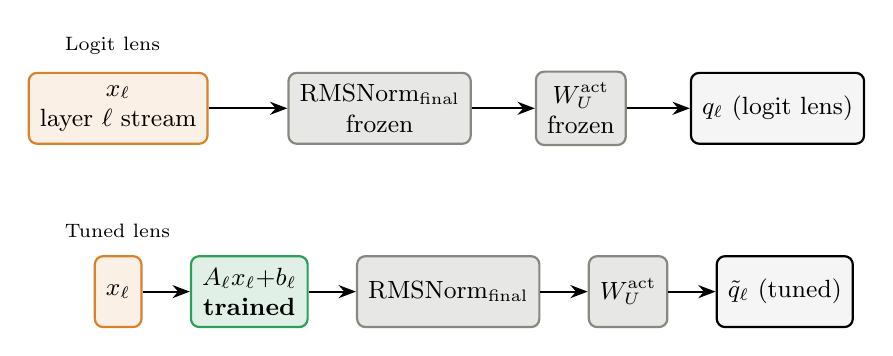
\begin{tikzpicture}[font=\small,
  box/.style={draw,rounded corners=3pt,thick,minimum height=9mm,align=center,inner sep=4pt},
  arr/.style={-{Stealth[length=2.2mm]},thick}]
\node[box,fill=llm!12,draw=llm] (x) {$x_\ell$\\layer $\ell$ stream};
\node[box,fill=frz!20,draw=frz,right=10mm of x] (n1) {RMSNorm$_{\text{final}}$\\frozen};
\node[box,fill=frz!20,draw=frz,right=8mm of n1] (u1) {$W_U^{\text{act}}$\\frozen};
\node[box,fill=black!4,right=8mm of u1] (q1) {$q_\ell$ (logit lens)};
\draw[arr] (x) -- (n1); \draw[arr] (n1) -- (u1); \draw[arr] (u1) -- (q1);
\node[box,fill=llm!12,draw=llm,below=14mm of x] (x2) {$x_\ell$};
\node[box,fill=act!15,draw=act,right=6mm of x2] (t) {$A_\ell x_\ell{+}b_\ell$\\\textbf{trained}};
\node[box,fill=frz!20,draw=frz,right=6mm of t] (n2) {RMSNorm$_{\text{final}}$};
\node[box,fill=frz!20,draw=frz,right=6mm of n2] (u2) {$W_U^{\text{act}}$};
\node[box,fill=black!4,right=6mm of u2] (q2) {$\tilde q_\ell$ (tuned)};
\draw[arr] (x2) -- (t); \draw[arr] (t) -- (n2); \draw[arr] (n2) -- (u2); \draw[arr] (u2) -- (q2);
\node[above=1mm of x,font=\scriptsize,anchor=south west,xshift=-8mm] {Logit lens};
\node[above=1mm of x2,font=\scriptsize,anchor=south west,xshift=-8mm] {Tuned lens};
\end{tikzpicture}
\caption{The tuned lens inserts one trained affine map per layer before the frozen read-out. Gray = frozen OpenVLA parts, green = the only trainable parameters.}
\end{figure}

\subsection{The four design choices that make it a lens, not a new model}
\begin{enumerate}
  \item \textbf{Everything in OpenVLA is frozen}, including $W_U$ and the final norm. Only $A_\ell, b_\ell$ train.
  \item \textbf{Initialize at the logit lens}: $A_\ell = I$, $b_\ell = 0$. Before training, the tuned lens \emph{is} the logit lens. Training measures how far you have to move from it.
  \item \textbf{Distill, don't supervise.} The target is the model's \emph{own} final distribution $p$ at the same position, not the ground-truth action:
  \begin{equation}
  \mathcal{L}_\ell = \mathbb{E}_{\text{inputs}}\Big[\KL\big(p \,\|\, \tilde q_\ell\big)\Big] = \mathbb{E}\Big[\textstyle\sum_{b} p(b)\,\big(\log p(b) - \log \tilde q_\ell(b)\big)\Big].
  \end{equation}
  The lens is asked ``can you recover what \emph{this model} will say?'', not ``can you solve the robot task?''. That keeps it from learning information the model doesn't use.
  \item \textbf{Keep it affine.} A linear map plus bias can rotate, rescale, and shift a basis. It cannot do the multi-step nonlinear computation the remaining layers do. (A full $4096\times4096$ affine map is still quite powerful, which matters in Section~\ref{sec:capacity}.)
\end{enumerate}

\paragraph{KL direction.} $\KL(p\,\|\,\tilde q)$ heavily penalizes the lens for putting low probability on bins the final layer likes. It is the same direction as the KL in your run~2 analysis, so the numbers are directly comparable.

\paragraph{Original training recipe.} Belrose et al.\ trained translators with SGD + Nesterov momentum for 250 steps, learning rate 1.0 with linear decay, gradient clipping at 1, weight decay $10^{-3}$, and about $2^{18}$ tokens per step. A later note in the paper reports that the Muon optimizer reached much lower KL and calls the original lenses ``severely undertrained''. The practical lesson: train until held-out KL stops improving, not for a fixed number of steps.

\subsection{What the paper found}
\begin{itemize}
  \item Tuned-lens predictions are more accurate and much less biased than the logit lens's at every layer, on models up to 20B parameters.
  \item \textbf{Causal faithfulness:} directions that matter most to the tuned lens (found by ablation) are also the directions that matter most to the model's actual output (Spearman $\rho=0.89$ in their Pythia-410M test). The lens reads features the model really uses.
  \item \textbf{Prediction depth} (the layer after which the lens's top-1 stops changing, i.e.\ your ``settle layer'') became more meaningful with the tuned lens. It correlates better with how hard an example is.
\end{itemize}

\section{The family of trained read-outs}
\label{sec:capacity}

The tuned lens is one point on a spectrum. Moving down the table adds capacity: the read-out can find more, but it becomes harder to say whether it \emph{found} information or \emph{computed} it.

\begin{center}
\small
\begin{tabularx}{\linewidth}{@{}lllX@{}}
\toprule
Read-out & Trained params / layer & Target & Question it answers \\
\midrule
Logit lens & 0 & -- & Is the answer already in $W_U$'s format? \\
Bias-only lens & $b_\ell$ (4K) & final $p$ & \ldots after correcting a constant offset? \\
Low-rank tuned lens & $A_\ell = I + UV^\top$, rank $k$ & final $p$ & \ldots after a small change of basis? \\
Tuned lens (full affine) & $A_\ell, b_\ell$ (16.8M) & final $p$ & \ldots after any change of basis? \\
New unembedding per layer & $256\times4096$ (1M) & final $p$ & Is the final answer linearly decodable at all? \\
Linear probe (your ridge) & $4096\times k$ & ground truth & Is the true action / object position linearly decodable? \\
MLP probe & larger & ground truth & Is it decodable by \emph{any} simple network? \\
\bottomrule
\end{tabularx}
\end{center}

\begin{mental}[: capacity vs.\ selectivity]
A read-out with too little capacity misses information that is there: the logit lens's failure mode. A read-out with too much capacity ``finds'' information by computing it from raw ingredients: a deep probe can decode almost anything from almost any layer. Good practice is to report \emph{several} rungs of the ladder and draw conclusions only from patterns that hold across them.
\end{mental}

\paragraph{Tuned lens vs.\ your ridge probes.} Your \texttt{--mode probe} regresses the \emph{executed} action and object positions from each layer, with no $W_U$ involved. The tuned lens asks whether layer $\ell$ can be translated into the model's \emph{own} answer \emph{through $W_U$}. They answer different questions, and agreement between them is strong evidence:
\begin{itemize}
  \item Probe finds the action at layer 15, and so does the tuned lens: the action is computed by mid-depth (story B).
  \item Probe finds it at 15 but the tuned lens doesn't: the information exists but not in a form the model's read-out path uses yet.
  \item Neither finds it before layer 26: strong support for a real late computation (story A).
\end{itemize}

%=====================================================================
\part{Applying It to the Perception$\to$Action Question}
%=====================================================================

\section{The hypothesis, stated precisely}

From run~2 (logit lens, LIBERO-Spatial, 6{,}460 steps):
\begin{itemize}
  \item Movement dimensions ($x,y,z$, roll, pitch, yaw) only beat the most-common-bin baseline at layers 25--28. Median settle layer is 28--31.
  \item The gripper settles much earlier (median layer 21), but mostly for ``keep doing the same thing''. Gripper \emph{switches} form late.
  \item Early layers are confidently wrong, concentrated on a few default bins.
\end{itemize}
\textbf{Hypothesis:} layers $\lesssim 20$ do perception (scene and instruction), and the action is computed in the last $\sim$8 layers.
\textbf{What the tuned lens adds:} it separates ``action computed late'' (A) from ``action computed earlier but expressed late'' (B).

\section{Predicted outcomes}

\begin{figure}[h]
\centering
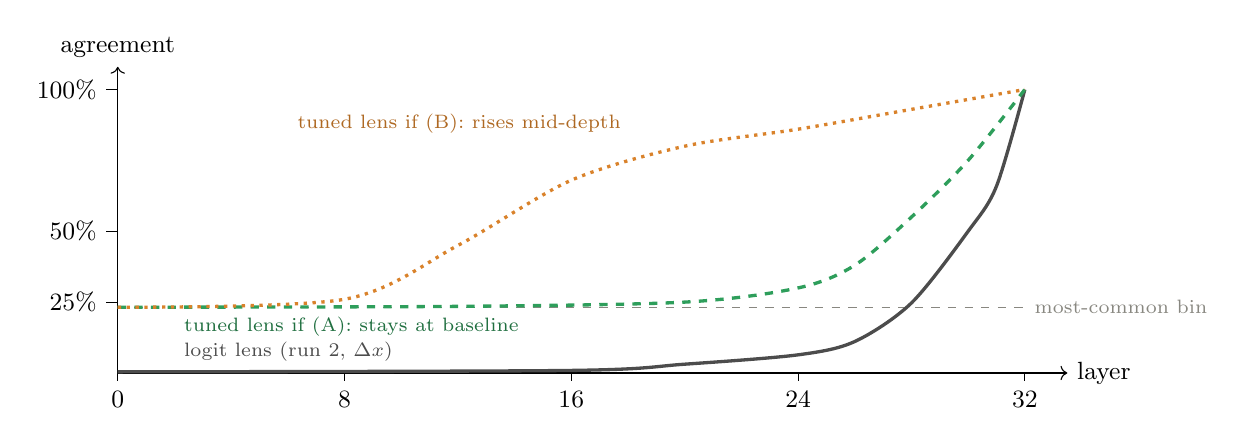
\begin{tikzpicture}[font=\small,x=0.36cm,y=3.6cm]
\draw[->] (0,0) -- (33.5,0) node[right] {layer};
\draw[->] (0,0) -- (0,1.08) node[above] {agreement};
\foreach \l in {0,8,16,24,32} \draw (\l,0) -- (\l,-0.03) node[below] {\l};
\foreach \v/\t in {0.25/25\%,0.5/50\%,1/100\%} \draw (0,\v) -- (-0.4,\v) node[left] {\t};
\draw[dashed,frz] (0,0.232) -- (32,0.232) node[right,font=\scriptsize] {most-common bin};
\draw[very thick,black!70] plot[smooth] coordinates {(0,0.004) (16,0.009) (20,0.031) (24,0.064) (26,0.111) (28,0.247) (30,0.5) (31,0.659) (32,1)};
\draw[very thick,act,dashed] plot[smooth] coordinates {(0,0.232) (12,0.235) (20,0.25) (24,0.3) (26,0.38) (28,0.55) (30,0.75) (32,1)};
\draw[very thick,llm,dotted] plot[smooth] coordinates {(0,0.232) (8,0.26) (12,0.45) (16,0.68) (20,0.8) (24,0.86) (28,0.93) (32,1)};
\node[font=\scriptsize,black!70,anchor=west] at (2,0.075) {logit lens (run 2, $\Delta x$)};
\node[font=\scriptsize,act!70!black,anchor=west] at (2,0.165) {tuned lens if (A): stays at baseline};
\node[font=\scriptsize,llm!80!black,anchor=west] at (6,0.88) {tuned lens if (B): rises mid-depth};
\end{tikzpicture}
\caption{Schematic only, not data. The black curve is the run~2 logit-lens agreement for $\Delta x$. Note that \emph{both} tuned-lens curves start at the most-common-bin baseline at layer 0: a trained bias alone can always output the most common bin. Beating the baseline is what counts, not beating the logit lens.}
\label{fig:outcomes}
\end{figure}

\begin{center}
\begin{tabularx}{\linewidth}{@{}lX@{}}
\toprule
Result & Interpretation \\
\midrule
Tuned lens $\approx$ baseline until $\sim$25, then rises & \textbf{(A) supported}, more strongly than before: even with a learned change of basis, the action isn't available mid-depth. \\
Tuned lens rises well above baseline by $\sim$15--20 & \textbf{(B)}: the action is mostly computed by mid-depth, and late layers re-express it for $W_U$. ``Split'' then describes representation format, not computation. \\
Low-rank lens $\approx$ full lens & The translation needed is simple (a few directions), and the conclusion doesn't depend on lens capacity. \\
Full lens $\gg$ low-rank lens at early layers & Be cautious: the full translator may be computing, not translating. Trust the low-rank result. \\
Gripper rises early, movement late & A per-dimension split, consistent with run~2's gripper finding. \\
\bottomrule
\end{tabularx}
\end{center}

\section{Specifics for OpenVLA}

\subsection{Which vocabulary to normalize over}
Two choices for the softmax:
\begin{itemize}
  \item \textbf{256 action rows only} (recommended, and what run~2 does). The question is ``which bin?''. It matches all your existing metrics.
  \item \textbf{Full 32064 vocabulary.} It also tests whether early layers would rather output a text token. That's interesting, but it mixes two questions.
\end{itemize}

\subsection{Which positions, and one translator or several}
Each simulator step has 7 read positions: the ``\texttt{\_}'' token for $\Delta x$, then each generated action token. The original tuned lens shares one translator per layer across all positions. For OpenVLA:
\begin{itemize}
  \item \textbf{Start with $\Delta x$ alone.} This is the data you already have (below).
  \item \textbf{Then all 7, with one shared translator per layer.} Seven times the training data per translator, and the most direct analogue of the paper.
  \item \textbf{Optionally one translator per (layer, dimension)}, if shared translators fit some dimensions much worse than others.
\end{itemize}

\subsection{The data you already have, and its limit}
\texttt{experiments.py} saves, for every step, the stream at \emph{all 33 layers} for the \emph{first} action position only (\texttt{rec["hidden"].append(hidden[0])}). So \texttt{runs/run2/hidden/*.npz} holds:
\[
H \in \mathbb{R}^{6460 \times 33 \times 4096}\ \text{(fp16, about 1.7 GB)}.
\]
\textbf{$\Delta x$ is ready to go.} The other six dimensions need a new run that also saves \texttt{hidden[1:7]}, about $7\times$ the storage ($\approx$12 GB).

\begin{pitfall}[: more parameters than examples]
A full translator has $4096^2 \approx 16.8$M parameters. With 5-fold episode-held-out splits, about 5{,}200 training vectors per layer remain. The full affine lens can therefore \emph{memorize} its training set. Its held-out score is the only number that means anything. Use some combination of:
\begin{itemize}
  \item \textbf{Low rank:} $A_\ell = I + U_\ell V_\ell^\top$ with rank $k\in\{8, 32, 128\}$, $V_\ell$ initialized to zero so training starts at the logit lens. Report results across $k$.
  \item \textbf{Weight decay toward identity:} penalize $\|A_\ell - I\|^2$, not $\|A_\ell\|^2$.
  \item \textbf{Early stopping} on held-out-episode KL.
  \item \textbf{More data:} more rollouts, and using all 7 positions with a shared translator.
\end{itemize}
\end{pitfall}

\section{Controls that make the result convincing}

\begin{enumerate}
  \item \textbf{Hold out whole episodes.} Consecutive steps are near-duplicates. Reuse the \texttt{GroupKFold}-by-episode split from \texttt{run\_probes}.
  \item \textbf{Layer-0 control.} At the $\Delta x$ read position, layer 0 is just the embedding of the ``\texttt{\_}'' token, \emph{identical at every step}. The tuned lens there can only output one fixed distribution, so its agreement must equal the most-common-bin rate (23.2\% for $x$ in run~2) and no more. A higher number means a bug or leakage.
  \item \textbf{Compare to the baseline, not to the logit lens.} As Figure~\ref{fig:outcomes} shows, a trained bias alone beats the logit lens at early layers. The meaningful line is the most-common-bin baseline.
  \item \textbf{Capacity sweep.} Bias-only, low-rank $k=8/32/128$, full. Draw conclusions only from what is stable across them.
  \item \textbf{Shuffled-input control.} Train on streams paired with targets from \emph{other} steps. Held-out agreement should fall to baseline. If it doesn't, the lens is exploiting something other than step-specific information.
  \item \textbf{Cross-check with probes.} Plot tuned-lens agreement next to your ridge-probe $R^2$ for the executed action at the same layers.
  \item \textbf{Causal follow-up (later).} A read-out shows information is \emph{present}. To show the model \emph{uses} it, intervene: patch or ablate the directions the translator relies on at layer $\ell$ and check whether the final action changes. This is the step that turns a correlation into a mechanism.
\end{enumerate}

\section{Implementation sketch}

\subsection{Targets and inputs}
\begin{lstlisting}
# H: [N, 33, 4096] fp16 from runs/run2/hidden/*.npz (Delta-x position)
# groups: [N] episode index, for GroupKFold  (load_hidden_dataset already does this)
norm, head = get_final_norm_and_head(model)          # frozen, as in --mode lens
W_act = head.weight[action_ids].float()              # [256, 4096], action rows of W_U

# Target: final distribution. hidden_states[32] is ALREADY normed in HF Llama.
with torch.no_grad():
    logp_final = torch.log_softmax(H[:, 32].float() @ W_act.T, dim=-1)   # [N, 256]
\end{lstlisting}

\subsection{A low-rank translator per layer}
\begin{lstlisting}
class Translator(nn.Module):
    def __init__(self, d=4096, rank=32):
        super().__init__()
        self.U = nn.Parameter(torch.randn(d, rank) / d**0.5)
        self.V = nn.Parameter(torch.zeros(rank, d))   # zero -> starts as the logit lens
        self.b = nn.Parameter(torch.zeros(d))
    def forward(self, x):                             # x: [B, d]
        return x + (x @ self.U) @ self.V + self.b     # A = I + U V

def lens_logp(x, translator):
    z = norm(translator(x))                           # frozen final RMSNorm
    return torch.log_softmax(z @ W_act.T, dim=-1)     # [B, 256]

# KL(p_final || q_lens), averaged over the batch
def kl(logp_final, logq):
    return (logp_final.exp() * (logp_final - logq)).sum(-1).mean()
\end{lstlisting}

\subsection{Training loop for one layer and one fold}
\begin{lstlisting}
for layer in range(32):                               # layer 32 needs no lens
    for train_idx, test_idx in GroupKFold(5).split(H, groups=groups):
        T = Translator(rank=k).cuda()
        opt = torch.optim.AdamW(T.parameters(), lr=1e-3, weight_decay=0.0)
        for epoch in range(max_epochs):
            for batch in minibatches(train_idx, 256):
                x = H[batch, layer].float().cuda()
                loss = kl(logp_final[batch], lens_logp(x, T))
                opt.zero_grad(); loss.backward(); opt.step()
            # early stopping on a validation split carved from train_idx
        # score on held-out episodes: agreement, +-k bins, KL, entropy
\end{lstlisting}
The OpenVLA weights are only needed to fetch $W_U^{\text{act}}$ and the final norm, so training runs on cached vectors and is cheap: minutes per layer on one GPU. Output the same metrics and plots as \texttt{--mode lens} so the curves overlay directly.

\section{The two-minute spoken explanation}

\begin{quote}
``The logit lens reads intermediate layers through OpenVLA's own output matrix. That assumes every layer stores information in the same format as the final layer, and nothing guarantees it. Our run~2 lens says movement actions only become readable around layer 26. That could mean the action is computed late, or that it's computed earlier but in a format the output matrix can't read. To separate those, I train a tuned lens: a small affine translator per layer, initialized to the identity, that maps that layer's residual stream into the final layer's format before the frozen output matrix reads it. The model stays completely frozen, and the translator is trained to match the model's own final prediction, not the true action, so it can't learn the task by itself. If the tuned lens still can't beat the most-common-bin baseline until the late layers, that's much stronger evidence that the action really is computed late. If it reads the action from mid-depth, the late layers are mostly translating. Controls: episode-held-out evaluation, a layer-0 sanity check, low-rank versions to limit capacity, and a comparison with linear probes on the true actions.''
\end{quote}

\section{Self-test questions}

\begin{enumerate}
  \item What is the difference between fine-tuning OpenVLA and fine-tuning a lens? Which one changes the model?
  \item In LoRA, why is $B$ initialized to zero? What does merging do, and why does it make inference no slower?
  \item How many trainable parameters does LoRA $r=32$ add to one $4096\times11008$ matrix?
  \item Why might the LIBERO checkpoint share its $W_U$ with base OpenVLA, and how would you check?
  \item State the two stories (A and B) the logit lens can't distinguish.
  \item Why is the tuned lens trained against the model's final distribution rather than the ground-truth action?
  \item Why does the tuned lens at layer 0 already score the most-common-bin rate, and why does that make ``beats the logit lens'' a weak claim?
  \item With about 5{,}200 training vectors and 16.8M translator parameters, what goes wrong, and what are three remedies?
  \item How would you tell whether a tuned lens is translating or computing?
  \item What experiment would show the model \emph{uses} the information a lens finds?
\end{enumerate}

\section{Sources}

\begin{thebibliography}{9}
\bibitem{belrose2023tuned} N.~Belrose, I.~Ostrovsky, L.~McKinney, Z.~Furman, L.~Smith, D.~Halawi, S.~Biderman, J.~Steinhardt.
\emph{Eliciting Latent Predictions from Transformers with the Tuned Lens.} arXiv:2303.08112, 2023 (v6, 2025). \url{https://arxiv.org/abs/2303.08112}

\bibitem{hu2021lora} E.~J. Hu, Y.~Shen, P.~Wallis, Z.~Allen-Zhu, Y.~Li, S.~Wang, L.~Wang, W.~Chen.
\emph{LoRA: Low-Rank Adaptation of Large Language Models.} ICLR 2022. \url{https://arxiv.org/abs/2106.09685}

\bibitem{kim2024openvla} M.~J. Kim, K.~Pertsch, S.~Karamcheti, et al.
\emph{OpenVLA: An Open-Source Vision-Language-Action Model.} CoRL 2024. \url{https://arxiv.org/abs/2406.09246}

\bibitem{peft} Hugging Face PEFT documentation, LoRA developer guide (\texttt{target\_modules="all-linear"}, initialization, \texttt{merge\_and\_unload}). \url{https://huggingface.co/docs/peft/developer_guides/lora}

\bibitem{ovlaft} OpenVLA fine-tuning script, \texttt{vla-scripts/finetune.py}. \url{https://github.com/openvla/openvla}
\end{thebibliography}

\noindent\small Run~2 numbers come from \texttt{docs/run2\_logit\_lens\_analysis.md}. The implementation sketch is illustrative and has not been run. Learning rates and epoch counts are starting points to tune on held-out KL.

\end{document}
